\documentclass{beamer}
\mode<presentation>
\usetheme{CambridgeUS}
\usepackage[russian]{babel}
\usepackage[utf8]{inputenc}
\usepackage[T2A]{fontenc}
\usepackage{sansmathaccent}
\pdfmapfile{+sansmathaccent.map}
\title[Звуковая волна]{Физические основы возникновения и распространения звуковых волн}
\author{Наумов Д.А.}
\date[09.01.2014] {Компьютерные музыкальные технологии и звуковой дизайн, 2014}

\begin{document}

%ТИТУЛЬНЫЙ СЛАЙД
\begin{frame}
  \titlepage
\end{frame}
  
%СОДЕРЖАНИЕ ЛЕКЦИИ
\begin{frame}
  \frametitle{Содержание лекции}
  \tableofcontents  
\end{frame}
  
%РАЗДЕЛ 1
\section{Физика образования и распространения звуковых волн}
\subsection{Природа звуковой волны}
\begin{frame}
Понятие "<звук"> может быть рассмотрено с двух принципиально различных позиций.
\begin{itemize}
\item Звук как {\itshape физическое явление}~--- это волнообразно распространяющиеся колебания частиц   упругой среды. Другими словами, звук есть результат колебательного процесса, распространяющегося в упругой среде, в частности~--- в воздушной среде.
\pause
\item Звук как {\itshape физиологическое явление}~--- это специфическое ощущение, вызываемое действием звуковых волн, распространяющихся в воздушной среде, на орган слуха.
\end{itemize}
\end{frame}
\begin{frame}
Некоторые факты о звуке:
\begin{itemize}
\item Звук может распространяться только в упругой среде. 
\pause
\item Источником источником звука может служить любое тело, способное совершать упругие колебания.  
\pause
\item Упругие периодические механические колебания источника звука вызывают колебания близлежащих к источнику частиц упругой среды, что приводит к периодическому сжатию (сгущению) и разрежению среды в этом месте. 
\pause
\item Избыточное давление воздействует ("<толкает">) на соседние слои (элементы объема) упругой среды, которые, в свою очередь, сжимаются, и возникает избыточное давление, которое воздействует на соседний слой среды, и т.д. 
\pause
\item Продольная волна представляет собой чередование сгущений (уплотнений) и разрежений в упругой среде в направлении перемещения волны.
\item Звуковые волны~--- суть продольные волны.
\end{itemize}
\end{frame}   

\subsection{Распространение звуковых волн}
\begin{frame}
Звук, который мы слышим,~--- это сложное явление. Звуковая волна, создающая давление на барабанную перепонку уха, является результирующей звуковой волной от нескольких источников, звуковые волны которых накладываются друг на друга, отражаются, преломляются и поглощаются на своем пути.
\begin{enumerate}
\item интерференция
\item отражение и преломление
\item поглощение и рассеяние
\item волновое движение в замкнутом объеме
\item дифракция
\item резонанс
\item эффект Доплера
\end{enumerate}
\end{frame}

\begin{frame}
Явление {\itshape интерференции} во времени базируется на известном принципе суперпозиции волн, смысл которого сводится к следующему: если в среде одновременно распространяется система $n$ различных волн, то каждая из волн распространяется независимо от других. При этом результирующие скорость, смещение, ускорение каждой частицы среды равны векторным суммам соответствующих величин, обусловленных каждой из волн порознь.
\begin{figure}[h]
\centering
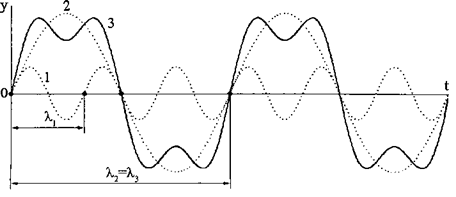
\includegraphics[scale=0.8]{pic-interferention-01}
\end{figure}
\end{frame}

\begin{frame}
\begin{block}{Сумма двух колебаний одинаковой частоты, амплитуды и фазы}
\begin{center}
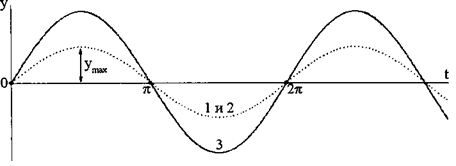
\includegraphics[scale=0.8]{pic-interferention-02}
\end{center}
\end{block}
\begin{block}{Сумма колебаний одинаковой частоты и амплитуды и разностью фаз \(\pi\)}
\begin{center}
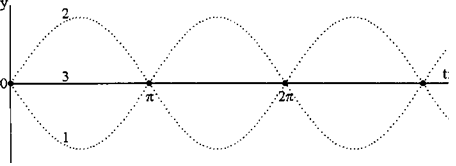
\includegraphics[scale=0.8]{pic-interferention-03}
\end{center}
\end{block}
\end{frame}

\begin{frame}
\begin{block}{Биение}
\begin{center}
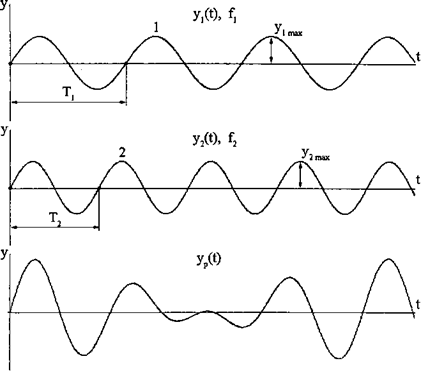
\includegraphics[scale=0.8]{pic-interferention-04}
\end{center}
\end{block}
\end{frame}

\begin{frame}
\begin{block}{Отражение и преломление}
\begin{center}
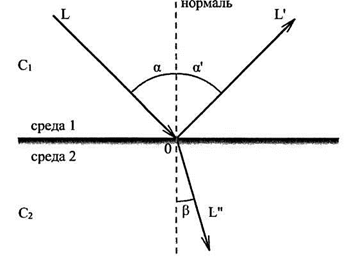
\includegraphics[scale=0.8]{pic-reflection-01}
\end{center}
\end{block}
\end{frame}
\begin{frame}
\begin{block}{Поглощение}
Энергия звуковой волны в процессе ее распространения поглощается средой. Этот эффект называют {\itshape поглощением звуковых волн}. Существование эффекта поглощения обусловлено процессами теплообмена и межмолекулярного взаимодействия в среде, точнее~--- внутренним трением и теплопроводностью.
\end{block}
\begin{block}{Рассеяние}
{\itshape Рассеяние звука} возникает в результате взаимодействия звуковой волны со встречающимися на ее пути многочисленными препятствиями (встречные потоки воздуха, завихрения, ветер). 
В результате столкновения с этими препятствиями звуковая волна как бы "<рассыпается"> на множество волн, которые распространяются во всевозможных направлениях.
\end{block}
\end{frame}

\begin{frame}
Звук, идущий от источника, расположенного в закрытом помещении, многократно ударяясь и отражаясь от стен помещения, воспринимается слушателем как звук, сопровождающийся специфическим гулом~--- {\itshape реверберацией}.
\begin{center}
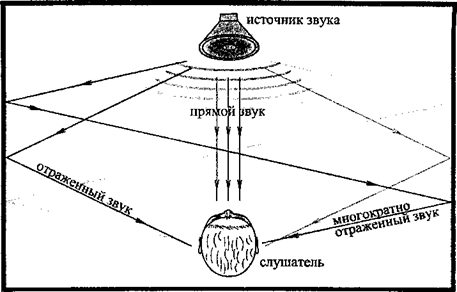
\includegraphics[scale=0.8]{pic-reverberation-01}
\end{center}
\end{frame}

\begin{frame}
\begin{block}{Дифракция}
способность волн огибать малые препятствия.
\end{block}
\begin{block}{Резонанс}
эффект резкого возрастания амплитуды вынужденных колебаний какой-то упругой системы при близком приближении или полном совпадении частоты вынужденных колебаний с собственной частотой этой системы.
\end{block}
\begin{block}{Эффект Доплера}
зависимость частоты колебаний, воспринимаемых приемником, от скоростей движения источника волн и приемника по отношению к среде, в которой распространяется звуковая волна.
\end{block}
\end{frame}

\begin{frame}
\begin{center}
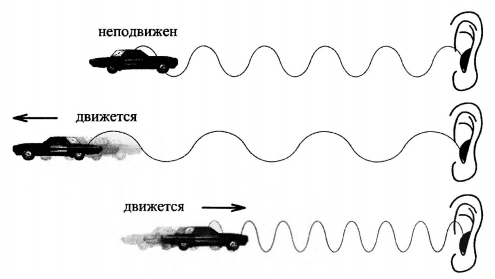
\includegraphics[scale=0.9]{pic-dopler-01}
\end{center}
\end{frame}
  
%РАЗДЕЛ 2
\section{Математическое представление звуковой волны}
\subsection{Уравнение звуковой волны}
\begin{frame}
Звуковые колебания называются {\itshape периодическими}, если значения физических величин, изменяющихся в процессе колебаний, повторяются через  равные промежутки времени~--- период колебания \(T\). В непериодических звуковых колебаниях отсутствует отсутствует периодическая повторяемость физических величин, изменяющихся в процессе колебания.
\begin{block}{Простейшее гармоническое колебание}
\begin{center}
\(y(t)=A\sin(\omega t+\varphi)\)
\end{center}
\begin{itemize}
\item \(y(t)\)~--- обозначение физической величины, которая изменяется в функции времени по синусоидальному закону;
\item \(A\)~--- амплитуда колебания, т.е. максимальное значение функции \(у(t)\);
\item \(\omega=2\pi f=\frac{2\pi}{T}\)~--- угловая (циклическая) частота колебаний;
\item \(f\)~--- частота колебаний;
\item \(\varphi\)~--- начальная фаза колебаний.
\end{itemize}
\end{block}
\end{frame}  

\begin{frame}
\begin{block}{Спектр звукового сигнала}
совокупность составляющих синусоидальных звуковых волн, в результате наложения которых получается исходная результирующая звуковая волна. 
\end{block}
Совокупность (набор) значений амплитуд и частот составляющих синусоидальных волн называется соответственно спектром амплитуд и спектром частот.
\begin{block}{Уравнение звуковой волны}
описывает колебания всех частиц (точек) звуковой волны, расположенных на любых расстояниях \(х\) по отношению к начальной точке. 
\[y(t) = A\sin[2\pi(\frac{t}{T}-\frac{\Delta t}{T})] = A\sin[2\pi(\frac{t}{T}-\frac{x}{CT})]=A\sin[2\pi(\frac{t}{T}-\frac{x}{\lambda})]\]
где \(\lambda\)~--- длина звуковой волны.
\end{block}
\end{frame}

\subsection{Графический способ отображения звуковых сигналов}
\begin{frame}
Cпособ графического отображения звукового сигнала в виде значений его уровня (амплитуды) во времени называют {\itshape амплитудно-временным}.
\begin{block}{Сигналлограмма}
график, отображающий зависимость амплитуды текущего звукового сигнала в функции времени.
\end{block}
\begin{center}
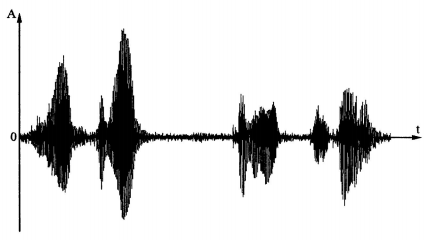
\includegraphics[scale=0.8]{pic-waveform-01}
\end{center}
\end{frame}    

\begin{frame}
Если очертить сигналограмму сверху и снизу таким образом, что изображенные на ней колебания окажутся "<вписанными"> между очерчивающими их линиями, то в результате получится {\itshape график амплитудной огибающей сигнала}.
\begin{center}
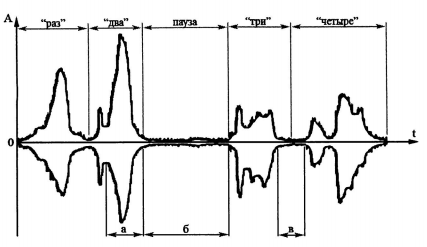
\includegraphics[scale=0.8]{pic-waveform-02}
\end{center}
\end{frame}  

\begin{frame}
\begin{center}
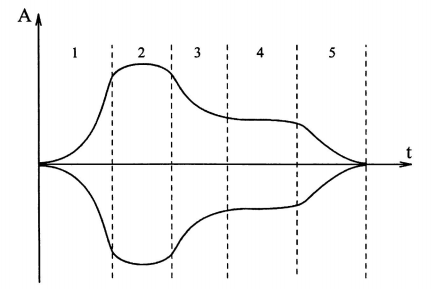
\includegraphics[scale=0.7]{pic-waveform-03}
\end{center}
\begin{enumerate}
\item Атака, подъем (от англ. "<attack">).
\item Стабилизация (от англ. "<hold">).
\item Спад (от англ. "<decay">).
\item Удержание (от англ. "<sustain">).
\item Затухание (от англ. "<release">).
\end{enumerate}
\end{frame}  

\begin{frame}
\begin{block}{Пример сигналлограммы короткого звука виолончели}
\begin{center}
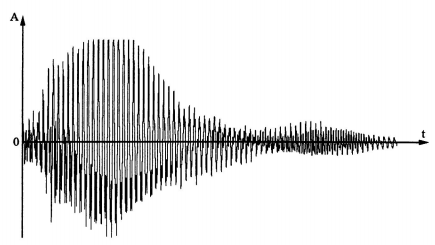
\includegraphics[scale=0.8]{pic-waveform-04}
\end{center}
\end{block}
\end{frame} 

\begin{frame}
\begin{block}{График амплитудно-частотного спектра}
график амплитудно-частотной зависимости, на котором по оси абсцисс откладываются частоты составляющих спектра, а по оси ординат~--- амплитуды соответствующих частотных составляющих. 
\begin{center}
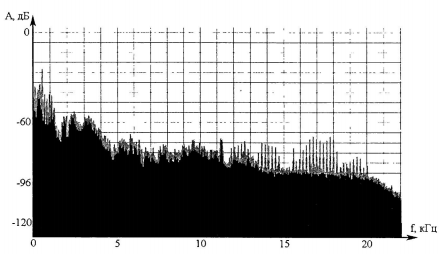
\includegraphics[scale=0.8]{pic-specter-01}
\end{center}
\end{block}
\end{frame} 

\begin{frame}
\begin{block}{Спектрограмма}
псевдо-трехмерный график в прямоугольной системе координат, на котором по оси \(X\) откладывается время, по оси \(Y\)~--- частота, а амплитуды частотных составляющих изображаются в соответствующих точках графика насыщенностью цвета.
\begin{center}
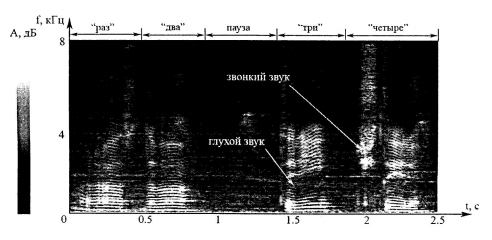
\includegraphics[scale=0.8]{pic-specter-02}
\end{center}
\end{block}
\end{frame} 

\begin{frame}
\begin{block}{Трехмерное представление спектрограммы}
\begin{center}
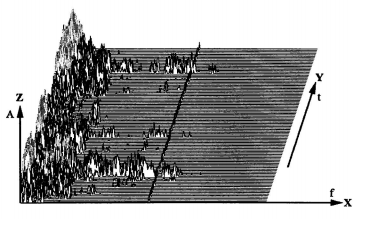
\includegraphics[scale=1.0]{pic-specter-03}
\end{center}
\end{block}
\end{frame} 

\subsection{Основные понятия гармонического анализа}

\begin{frame}
\begin{block}{Суть гармонического анализа}
любое периодическое колебание с частотой \(\omega\) можно представить в виде суммы гармонических колебаний, и наоборот, зная параметры отдельных гармоник (амплитуду, частоту и начальную фазу), можно с помощью их тригонометрического суммирования получить (или приближенно смоделировать) результирующее колебание. 
\end{block}
Любую сложную периодическую функцию можно разложить в тригонометрический гармонический ряд (называемый рядом Фурье) и анализировать эту функцию при помощи гармонического анализа, т.е. анализа гармоник, составляющих эту результирующую функцию. 
\begin{block}{Ряд Фурье для временной периодической функции}
\[ y(t) \approx \frac{a_0}{2} + \sum\limits_{v=1}^{\infty}(a_v\cos(v\omega t) + b_v\sin(v\omega t)),\]
\end{block}
\end{frame}

\begin{frame}
\begin{itemize}
\item Сумма гармонических колебаний с периодами \(T_1, \frac{1}{2}T_1, \frac{1}{3}T_1,...,\frac{1}{v}T_1\), где \(\frac{1}{v}T_1=T_v\)~--- период \(v\)-ой гармоники дает результирующее колебание с периодом \(T_1\). Это правило относится и к частотам \(\omega\), а именно: сумма любого числа гармонических колебаний с частотами, кратными \(\omega_1\), т.е. \(\omega_1, 2\omega_1,3\omega_1,...,v\omega_1\) дает результирующее колебание с частотой \(\omega_1\).
\pause
\item Угловая частота \(\omega_1=2\pi f_1\) называется {\itshape основной гармоникой} или {\itshape основной частотой}. Частоты \(\omega_2=2\omega_1, \omega_3=3\omega_1,...,\omega_v=v\omega_1\)~--- это {\itshape обертоны} или просто {\itshape гармоники} (говорят, "<вторая гармоника">, "<третья гармоника"> и т.д.).
\pause
\item Представление функции \(y(t)\) в виде суммы гармонических колебаний называется {\itshape разложением функции в спектр}. 
\end{itemize}
\end{frame}   

\begin{frame}
Качество музыкального (и немузыкального) звука зависит от состава его частотного спектра и правильного выбора пропорций частот, входящих в этот спектр. 

"<Качество"> определяется: 
\begin{enumerate}
\item относительным количеством различных гармоник в спектре звука;
\item относительными значениями коэффициентов ряда Фурье, которые указывают, с "<каким весом"> каждая гармоника входит в общее колебание (т.е. в результирующую функцию). 
\end{enumerate}
\begin{block}{Тембровая окраска звука} 
определяется распределением интенсивности обертонов (высших гармоник). 
\end{block}
Камертон может обеспечить практически чистый тон. Все музыкальные и немузыкальные звуки, не говоря уже о звуковых шумах, имеют широкий частотный спектр. 
Один и тот же музыкальный тон, взятый на разных инструментах, будет иметь одну и ту же основную частоту, но разные частотные спектры, т.е. разный {\itshape тембр}. 
\end{frame}  

\subsection{Гармонический анализ реальных звуковых сигналов}
\begin{frame}
\begin{itemize}
\item Для получения частотного спектра сигнала, описанного его дискретными значениями, применяют {\itshape дискретное преобразование Фурье}, или {\itshape ДПФ},~--- специально созданную разновидность преобразования Фурье, предназначенную для спектрального разложения дискретных сигналов.
\pause
\item Чтобы сделать вычисления ДПФ в цифровой вычислительной технике более эффективными, был создан алгоритм, названный быстрым преобразованием Фурье, или БПФ (Fast Fourier Transform~--- FFT).
\pause
\item С использованием ДПФ звуковой сигнал, описанный дискретными численными значениями, может быть представлен в виде амплитудно-частотного спектра. Любой, даже самый сложный по форме сигнал (например, звук голоса человека), можно представить суммой простейших синусоидальных колебаний определенных частот и амплитуд. 
\end{itemize}
\end{frame}    

\begin{frame}
\begin{block}{Сигналограмма фрагмента музыкальной аудиозаписи продолжительностью 0.25с}
\begin{center}
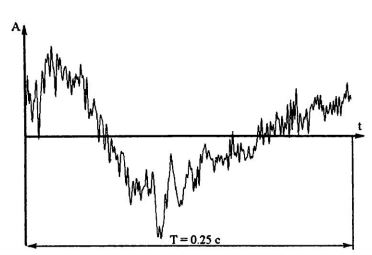
\includegraphics{pic-specter-04}
\end{center}
\end{block}
\end{frame} 

\begin{frame}
\begin{block}{Сигналограмма аудиофрагмента и график частичной суммы S(x,1)}
\begin{center}
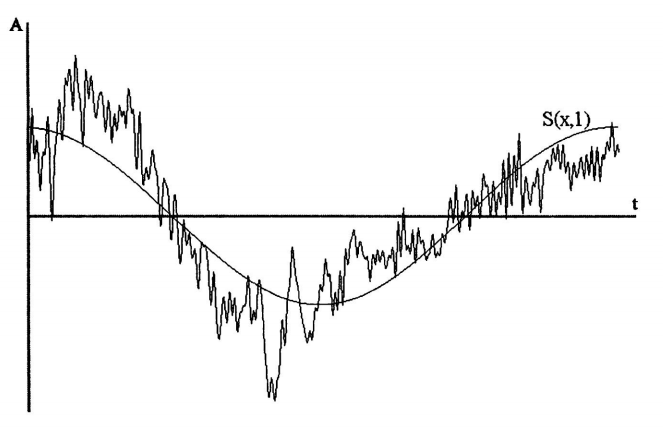
\includegraphics[scale=0.6]{pic-specter-05}
\end{center}
\end{block}
\end{frame} 

\begin{frame}
\begin{block}{Сигналограмма аудиофрагмента и график частичной суммы S(x,2)}
\begin{center}
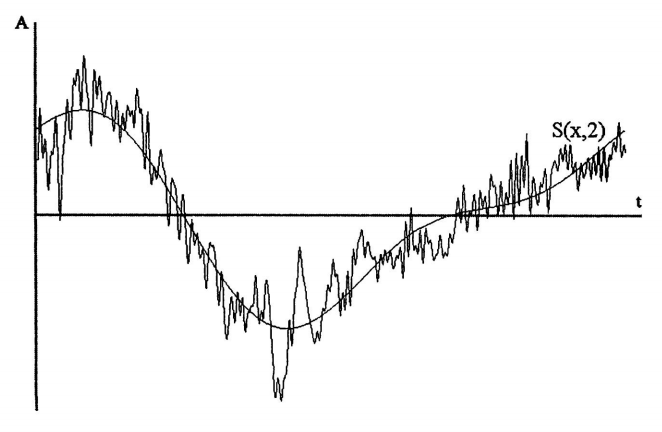
\includegraphics[scale=0.6]{pic-specter-06}
\end{center}
\end{block}
\end{frame} 

\begin{frame}
\begin{block}{Сигналограмма аудиофрагмента и график частичной суммы S(x,15)}
\begin{center}
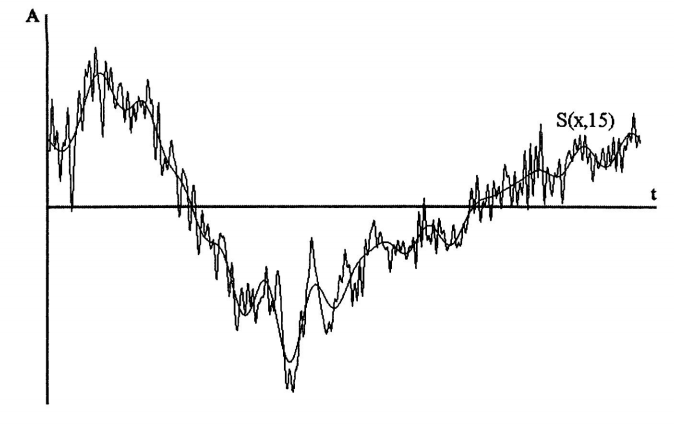
\includegraphics[scale=0.6]{pic-specter-07}
\end{center}
\end{block}
\end{frame} 

\begin{frame}
\begin{block}{Сигналограмма аудиофрагмента и график частичной суммы S(x,40)}
\begin{center}
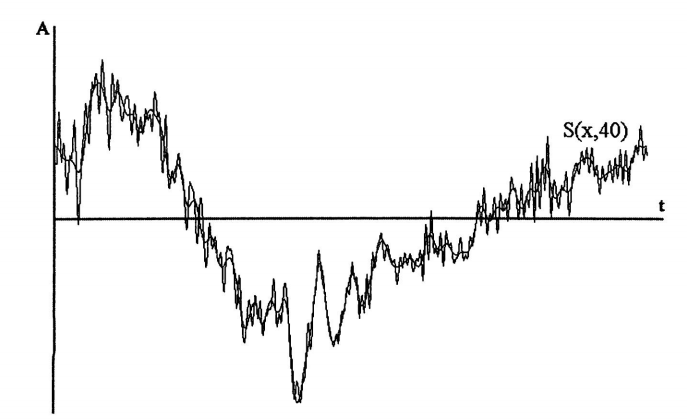
\includegraphics[scale=0.6]{pic-specter-08}
\end{center}
\end{block}
\end{frame} 

\begin{frame}
\begin{block}{Полный спектр анализируемого аудиофрагмента}
\begin{center}
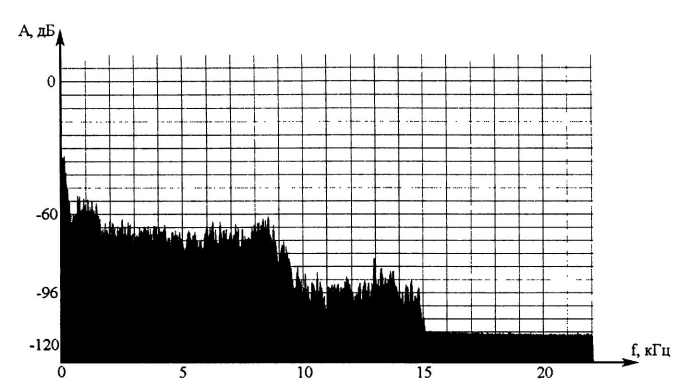
\includegraphics[scale=0.6]{pic-specter-09}
\end{center}
\end{block}
\end{frame} 

\subsection{Звуки различных источников}
\begin{frame}
Источник человеческого голоса, точнее~--- основной частоты голоса,~--- голосовые связки. 
\begin{block}{Сигналограмма звука "и"}
\begin{center}
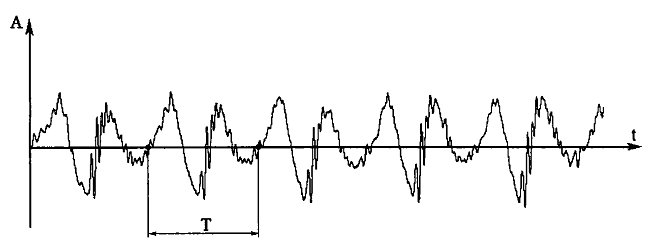
\includegraphics[scale=0.5]{pic-soundkind-01}
\end{center}
\end{block}
Основные частоты различных по типу голосов:
\begin{itemize}
  \item для баса: от 70 до 400 Гц;
  \item для баритона: от 110 до 440 Гц;
  \item для тенора: от 130 до 590 Гц;
  \item для контральто: от 175 до 780 Гц;
  \item для меццо-тинто: от 220 до 1050 Гц;
  \item для сопрано: от 350 до 1320 Гц.
\end{itemize}
\end{frame}   
   
\begin{frame}
При формировании звуков речи и пения, осуществляемом системой природных резонаторов речевого аппарата, подчеркиваются те или иные группы близлежащих частот их спектра. Cпектральных максимумов может быть четыре и больше, но распознавание каждого звука связано с одним или двумя первыми усиленными участками спектра~---{\itshape формантами}. 
\begin{block}{Частотное размещение формантных областей}
\begin{center}
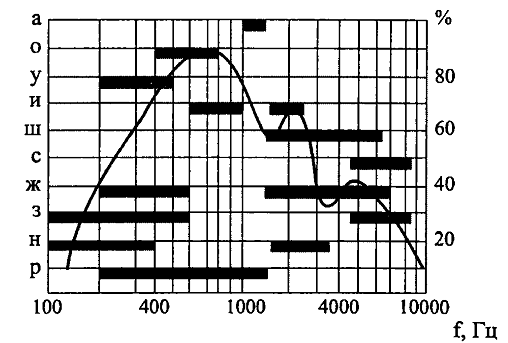
\includegraphics[scale=0.4]{pic-soundkind-02}
\end{center}
\end{block}
Для гласных звуков характерны форманты с дискретным спектром; для согласных~--- со сплошным.
\end{frame}   
   
\end{document}
